\subsection[Mainflux]{Wybrana platforma}
Mainflux umożliwia połączenie urządzeń do aplikacji oraz jednocześnie poprzez wykorzystanie JWT zapewnia bezpieczeństwo na wysokim poziomie. Tak jak zostało przedstawione w tabeli~\ref{tab:plat1}, mainflux oferuje wieloprotokołowy przekaźnik komunikatów, pozwala to na wybranie odpowiedniego protokołu do zapewnienia niezbędnych wymagań.
Mainflux jest używany jako oprogramowanie pośrednie to oznacza, że wykorzystuje serwer, który udostępnia funkcje oraz usługi potrzebne do stworzenia aplikacji IoT. Podstawowymi usługami są: 


\begin{itemize}
    \item Messaging bridge pośredniczy w wysyłaniu wiadomości pomiędzy urządzeniem a aplikacją. 
    \item User manager (Mainflux UI, Mainflux CLI) – umożliwia użytkownikowi zarządzanie zasobami. Pierwszy sposób to zarządzanie przez stronę internetową (Mainflux UI). Aby użytkownik mógł zarządzać zasobami musi się zalogować na stronie, po czym ma możliwość dodawania, usuwania, edycji rzeczy oraz łączenia kanałów z rzeczami. Drugim sposobem jest bootstraping (Mainflux CLI) czyli zautomatyzowane zarządzanie zasobami, wykorzystując bootstraping rejestracja nowych urządzeń może odbywać się bez udziału człowieka.
    \item Normalizer służy do zmieniania struktury wiadomości. Mainflux może otrzymywać wiadomości, w różnych formatach. Normalizer zmienia przesłaną wiadomość na format SenML (Sensor Markup Language), po czym przekazuje ją do zapisania w bazie danych.
    \item NATS otrzymuje wiadomości od rzeczy i może automatycznie reagować na przesłane dane, w oparci o konfigurowalny zestaw reguł.
    \item Writer służy do zapisywania komunikatów w bazie danych. Ponieważ istnieje wiele różnych systemów baz danych, dla każdego z nich musi istnieć odpowiedni moduł piszący​.
\end{itemize}

Poniższy schemat pokazuje zależności między tymi usługami.

\begin{figure}[H]
    \centering
    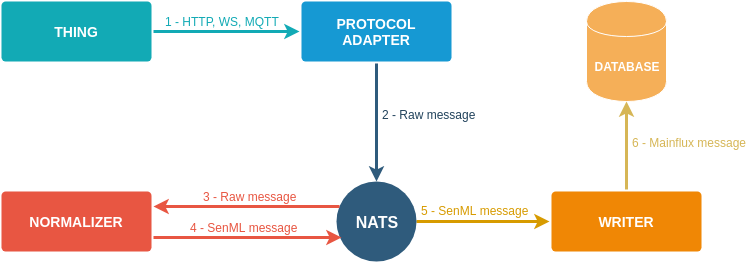
\includegraphics[width=\textwidth]{kp03}
    \caption{Placeholder}
    \label{fig:iotarch}
\end{figure}
//https://medium.com/mainflux-iot-platform/mainflux-open-source-iot-platform-set-up-and-usage-70bed698791a pozniej dodam do zrodel 

Aby zrozumieć jak działa przesyłanie wiadomości za pośrednictwem platformy mainflux trzeba poznać trzy podstawowe koncepty jakie zostały wprowadzone.
\begin{itemize}
    \item Użytkownik reprezentuje człowieka w systemie, który jest identyfikowany za pomocą danych do logowania jest on używany do zarządzania innymi zasobami. Zarządzanie obejmuje tworzenie, edytowanie oraz usuwanie rzeczy  i kanałów, a także do łączenia rzeczy z kanałami. 
    \item Rzecz reprezentuje urządzenie lub aplikację każda rzecz posiada identyfikator oraz klucz dodatkowo, może mieć przypisany typ (aplikacja, urządzenie). 
    \item Kanał pozwala na połączenia rzeczy między sobą. Każdy kanał ma swoje id, do kanału może być podłączonych więcej niż 2 rzeczy, każdy kto nasłuchuje na danym kanale otrzymuje tą wiadomość.
\end{itemize}

